%!TEX program = xelatex 
%%%%%%%%%%%%%%%%%%%%%%%%%%%%%%%%%%%%%%%%%%%%%%%%%%
% 载入模版
%
% 载入 hutbthesis.cls文件定义的模板
%%%%%%%%%%%%%%%%%%%%%%%%%%%%%%%%%%%%%%%%%%%%%%%%%%

\documentclass[AutoFakeBold]{hutbthesis}
\addbibresource{content/reference.bib}

%%%%%%%%%%%%%%%%%%%%%%%%%%%%%%%%%%%%%%%%%%%%%%%%%%
% 基本信息
%
% 用户自行输入标题、作者等基本信息
% 都存储在\content\info.tex文件中
%%%%%%%%%%%%%%%%%%%%%%%%%%%%%%%%%%%%%%%%%%%%%%%%%%
%!TEX root = ../hutbthesis_main.tex
% 文章信息
\titlecn{湖南工商大学学位论文 } 
\titleen{Hunan University of Technology and Business Thesis \LaTeX{} Template v0.1}


%\minormajor{通信工程}
%\interestmajor{通信工程}
\author{张三}
\subsupervisor{}
\studentid{2212223334}
\priormajor{通信工程}
\myclass{通信工程2201班}
\supervisor{王五\ 教授}
\department{智能工程与智能制造学院}
\thesisdate{year=2023, month=5}

%以下的对本科生没有用
\clcnumber{TP391} 				% 中图分类号 Chinese Library Classification
\schoolcode{10533}			% 学校代码
\udc{004.9}						% UDC
\academiccategory{学术学位}	% 学术类别



\begin{document}
%%%%%%%%%%%%%%%%%%%%%%%%%%%%%%%%%%%%%%%%%%%%%%%%%%
% 封面绘制
%
% 1.5版本重新编写了封面绘制宏,并用latex使用者更习惯的
% \maketitle代替之前的\makecoverpage
%%%%%%%%%%%%%%%%%%%%%%%%%%%%%%%%%%%%%%%%%%%%%%%%%%
\maketitle

%\declarationzh

% 启用大罗马字母进行编号
\frontmatter
% 设置页眉和页脚

%\include{content/info}

%!TEX root = ../hutbthesis_main.tex

\begin{declarationzh}
		
本人郑重声明:所呈交的本科毕业设计 \uline{ 湖南工商大学学位论文 \LaTeX{} 模板使用示例 v0.1 } 是本人在指导老师的指导下,独立进行研究工作所取得的成果,成果不存在知识产权争议,除文中已经注明引用的内容外,本设计不含任何其他个人或集体已经发表或撰写过的作品成果。
对本设计做出重要贡献的个人和集体均已在文中以明确方式标明。本人完全意识到本声明的法律结果由本人承担。
	
	\vspace{30pt}
	\begin{tabular}{ll}
		%\renewcommand{\arraystretch}{2}
		\hspace{240pt} \makebox[4em][s]{作者签名:} & \underline{\makebox[100pt][c]{  }} \\
		\hspace{240pt} \makebox[4em][s]{日\qquad 期:}	 &
		\underline{\makebox[100pt][c]{\qquad 年\quad 月\quad   日 }} \\
	\end{tabular}

	
	
\end{declarationzh}

%%%%%%%%%%%%%%%%%%%%%%%%%%%%%%%%%%%%%%%%%%%%%%%%%%
% 中文摘要
%
% 存储在\content\abstractzh.tex文件中
%%%%%%%%%%%%%%%%%%%%%%%%%%%%%%%%%%%%%%%%%%%%%%%%%%
%!TEX root = ../csuthesis_main.tex
% 设置中文摘要
\keywordscn{湖南工商大学\quad 学位论文\quad LaTeX模板}
%\categorycn{TP391}
\begin{abstractzh}

LaTeX利用设置好的模板,可以编译为格式统一的pdf。目前国内大多出版社与高校仍在使用word,word由于其强大的功能与灵活性,在新手面对形式固定的论文时,排版、编号、参考文献等简单事务反而会带来很多困难与麻烦,对于一些需要通篇修改的问题,要想达到LaTeX的效率,对word使用者来说需要具有较高的技能水平。

为了能把主要精力放在论文撰写上,许多国际期刊和高校都支持LaTeX的撰写与提交,新手不需要关心格式问题,只需要按部就班的使用少数符号标签,即可得到符合要求的文档。且在需要全篇格式修改时,更换或修改模板文件,即可直接重新编译为新的样式文档,这对于word新手使用word的感受来说是不可思议的。

本项目的目的是为了创建一个符合湖南工商大学本科生撰写规范的TeX模板,解决学位论文撰写时格式调整的痛点。


\end{abstractzh}

%%%%%%%%%%%%%%%%%%%%%%%%%%%%%%%%%%%%%%%%%%%%%%%%%%
% 英文摘要
%
% 存储在\content\abstracten.tex文件中
%%%%%%%%%%%%%%%%%%%%%%%%%%%%%%%%%%%%%%%%%%%%%%%%%%
%!TEX root = ../csuthesis_main.tex
\keywordsen{HUTB\ \ LaTeX\ \ Template}
\begin{abstracten}

LaTeX can be compiled into a pdf of uniform format using the set template.At present, most domestic publishers and universities still use word. Because of its powerful function and flexibility, when faced with fixed-form papers by novices, simple matters such as typesetting, numbering, and reference documents will bring many difficulties and troubles. For some problems that need to be modified throughout, to achieve the efficiency of LaTeX, it requires a high level of skill for word users.

In order to focus on the writing of papers, many international journals and universities support the writing and submission of LaTeX. Novices don't need to care about formatting issues. They only need to use a few symbolic labels step by step to get the documents that meet the requirements. And when you need to modify the entire format, you can directly recompile the template file by replacing or modifying the template file. This is incredible for the word novice to use the word.


\end{abstracten}


%%%%%%%%%%%%%%%%%%%%%%%%%%%%%%%%%%%%%%%%%%%%%%%%%%
% 目录
%
% 使用重定义的tableofcontents宏绘制目录
% 满足学校的样式要求
%%%%%%%%%%%%%%%%%%%%%%%%%%%%%%%%%%%%%%%%%%%%%%%%%%
\tableofcontents


% 启用数字编号,改为第 x 页  共 x 页格式
\mainmatter

%%%%%%%%%%%%%%%%%%%%%%%%%%%%%%%%%%%%%%%%%%%%%%%%%%
% 正文
%
% 存储在\content\content.tex文件中
%%%%%%%%%%%%%%%%%%%%%%%%%%%%%%%%%%%%%%%%%%%%%%%%%%
% 正文
%%!TEX root = ../hutbthesis_main.tex

%子章节为了便于查找和修改,建议通过input拆分文件

%%%%%%%%%%%%%%%%%%%%%%%%%%%%%%%%绪论%%%%%%%%%%%%%%%%
%!TEX root = ../../csuthesis_main.tex
\chapter{一级标题}

这是湖南工商大学学位论文\LaTeX{}模板,下面的文字主要作用为对重构后的模板样式设置进行测试。
测试样例基本覆盖模板设定,包括多级标题的基本样式,段落与缩进距离。

\section{二级标题}

\subsection{三级标题}

\subsubsection{四级标题}

一级标题根据学校提供的Word模板要求,三号黑体居中,上下各空一行,章节号空一个汉字,
并且每一章节单独起一页,章节号格式应使用阿拉伯数字而非中文汉字。

二级标题为小四号黑体,缩进两个汉字。章节号后空一个汉字。

三级标题小四号楷体GB2312,字体包含在项目中,同样缩进两个汉字,章节号后空一个汉字。

四级标题参照本科学术论文设计样式,分项采取(1)、(2)、(3)的序号。

所有标题样式由\cls{undergraduate.cls}模板文件 \cs{ctexset} 进行设置。

\section{字体}

正文字体默认使用小四号宋体,英文为小四号 Times New Romen,各段行首缩进两个汉字

承千年文脉,扬湖湘精神。湖南工商大学坐落在历史文化名城长沙,创建于1949年,享有“经济湘军基地,企业名家摇篮”的盛誉。她是一所院士领衔的涵盖管理学、经济学、工学、理学、法学、文学、艺术学、交叉学科等多学科相互支撑、协调发展、特色鲜明的财经类大学,是湖南省本科一批招生高校、教育部本科教学工作水平评估优秀高校、博士学位授予立项建设单位、“十三五”国家产教融合发展工程应用型本科高校、全国首批百强“深化创新创业教育改革示范高校”、全国高校实践育人创新创业基地、教育部人文社会科学优秀成果奖大满贯高校。

学校拥有一批以中国工程院院士陈晓红为代表,包括国务院学位委员会管理科学与工程学科评议组召集人、国家自然科学基金委员会委员、教育部管理科学与工程类专业教学指导委员会副主任委员、教育部科技委管理学部副主任、国家基础科学中心主任、国家一级重点学科“管理科学与工程”和国家自然科学基金委创新研究群体负责人、教育部“长江学者创新团队”首席教授、国家“万人计划”领军人才、全国文化名家暨“四个一批”人才、国家首批“百千万人才工程”第一层次人选等在内的国家级高层次人才;拥有高级职称教师近500人,具有博士学位教师近800人;引智院士9名、“杰青”“长江”等专家学者和优秀企业家70人;院士团队入选“全国高校黄大年式教师团队”。

英文字体展示如下:

TeX (/tɛx, tɛk/, see below), stylized within the system as TEX, is a typesetting system (or a "formatting system") which was designed and mostly written by Donald Knuth\cite{knuth1984texbook} and released in 1978. TeX is a popular means of typesetting complex mathematical formulae; it has been noted as one of the most sophisticated digital typographical systems.


\subsection{调节字号}

可以使用 \cs{zihao}命令来调节字号。

\begin{tabular}{ll}
  \verb|\zihao{3} | & \zihao{3}  三号字 English \\
  \verb|\zihao{-3}| & \zihao{-3} 小三号 English \\
  \verb|\zihao{4} | & \zihao{4}  四号字 English \\
  \verb|\zihao{-4}| & \zihao{-4} 小四号 English \\
  \verb|\zihao{5} | & \zihao{5}  五号字 English \\
  \verb|\zihao{-5}| & \zihao{-5} 小五号 English \\
\end{tabular}

\subsection{调节字体}

需要说明的是由于学校写作指导要求的字体部分不可在Linux上使用,即便你的写作过程是在Linux或者macOS上完成的,
我们仍\textbf{强烈建议}您在Windows操作系统上编译最终版论文。

中文字体可以使用如下命令来调节。

\begin{tabular}{l l}
  \verb|\songti| & {\songti 宋体} \\
  \verb|\heiti| & {\heiti 黑体} \\
%   \verb|\kaiti| & {\kaiti 楷体}
\end{tabular}


\section{模板主要结构}

本项目模板的主要结构, 如下表所示:
% TODO 进一步完善

\begin{table}[ht]
  \centering
  \begin{tabular}{r|l|l}
    \hline\hline
    \multicolumn{2}{l|}{csuthesis\_main.tex } & 主文档,可以理解为文章入口。                                      \\ \hline
                                                & info.tex   & 作者、文章基本信息 \\ \cline{2-3}
                                                & abstactzh/en.tex    & 中/英文摘要内容 \\ \cline{2-3}
    \raisebox{1em}{content 目录 }          &  subchapters 目录   & 章节内容           \\ \hline
    \multicolumn{2}{l|}{images 目录}         & 用于存放图片文件                                                \\ \hline
    \multicolumn{2}{l|}{hutbthesis.cls }       & 模板入口                         \\ \hline\hline
  \end{tabular}
\end{table}

我们不建议模板使用者更改原有模板的结构,
但如果您确实需要,请务必先充分阅读本模板的使用说明并了解相应的\LaTeX{}模板设计知识。

%%%%%%%%%%%%%%%%%%%%%%%%%%%%%%%%绪论%%%%%%%%%%%%%%%%

%%%%%%%%%%%%%%%%%%%%%%%%%%%%%%%%图像插入示例%%%%%%%%%%%%%%%%
%!TEX root = ../../csuthesis_main.tex
\chapter{图表示例}

\section{图片与布局}

\subsection{插图}

图片可以通过\cs{includegraphics}指令插入,我们建议模板使用者将文章所需插入的图片源问卷放置在 images 目录中,
另外,矢量图片应使用PDF格式,位图照片则应使用JPG格式(LaTeX不支持TIFF格式)。具有透明背景的栅格图可以使用PNG格式。

下面是一个简单的插图示例。

\begin{figure}[hbt]
    \centering
    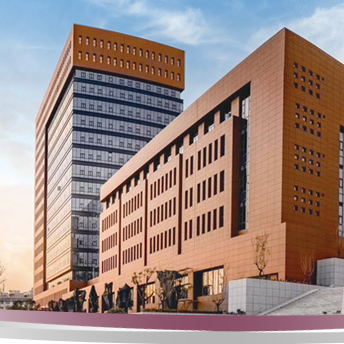
\includegraphics[width=0.3\linewidth]{hutb_building.png}
    \caption{插图示例}
    \label{f.example}
\end{figure}


如果一个图由多个分图(子图)组成,应通过(a),(b),(c)进行标识并附注在分图(子图下方)。
目前子图标识不居中问题没有解决,预计下个版本修复。

\subsection{横向布局}

模板提供常见的图片布局,比如单图布局\ref{f.example},另外还有横排布局如下:

\begin{figure}[!htb]
    \centering
    \begin{subfigure}[t]{0.24\linewidth}
        \begin{minipage}[b]{1\linewidth}
        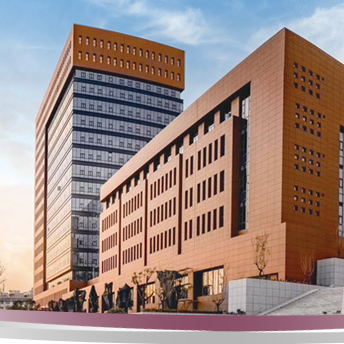
\includegraphics[width=1\linewidth]{hutb_building.png}
        \caption{test}
        \end{minipage}
    \end{subfigure}
    \begin{subfigure}[t]{0.24\linewidth}
        \begin{minipage}[b]{1\linewidth}
        \includegraphics[width=1\linewidth]{hutb_eim.png}
        \caption{test}
        \end{minipage}
    \end{subfigure}
    \begin{subfigure}[t]{0.24\linewidth}
        \begin{minipage}[b]{1\linewidth}
        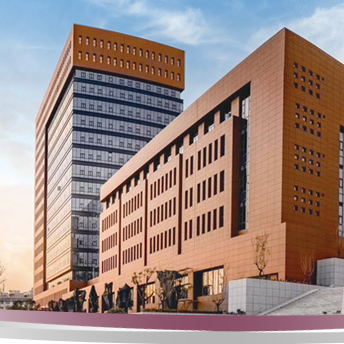
\includegraphics[width=1\linewidth]{hutb_building.png}
        \caption{test}
        \end{minipage}
    \end{subfigure}
    \begin{subfigure}[t]{0.24\linewidth}
        \begin{minipage}[b]{1\linewidth}
        \includegraphics[width=1\linewidth]{hutb_eim.png}
        \caption{test}
        \end{minipage}
    \end{subfigure}
    \caption{图片横排布局示例}
    \label{f.row}
\end{figure}

\section{纵向布局}

纵向布局如图\ref{f.col}

\begin{figure}[!htb]
    \centering
    \begin{subfigure}[t]{0.15\linewidth}
        \captionsetup{justification=centering} %ugly hacks
        \begin{minipage}[b]{1\linewidth}
        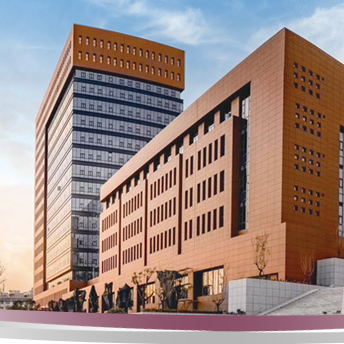
\includegraphics[width=1\linewidth]{hutb_building.png}
        \caption{test}
        \end{minipage}
    \end{subfigure}\\
    \begin{subfigure}[t]{0.15\linewidth}
        \captionsetup{justification=centering} %ugly hacks
        \begin{minipage}[b]{1\linewidth}
        \includegraphics[width=1\linewidth]{hutb_eim.png}
        \caption{test}
        \end{minipage}
    \end{subfigure}
    \caption{图片纵向布局示例}
    \label{f.col}
\end{figure}

\section{竖排多图横排布局}

\begin{figure}[!htb]
    \centering
    \begin{subfigure}[t]{0.13\linewidth}
        \captionsetup{justification=centering} 
        \begin{minipage}[b]{1\linewidth}
        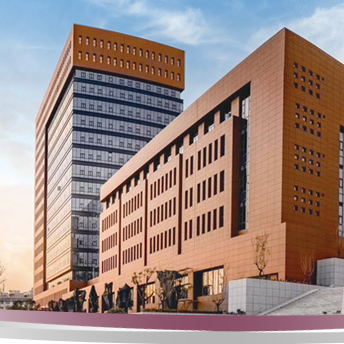
\includegraphics[width=1\linewidth]{hutb_building.png} 
        \vspace{-1ex} \vfill
        \includegraphics[width=1\linewidth]{hutb_eim.png}
        \caption{aaa}
        \end{minipage}
    \end{subfigure}
    \begin{subfigure}[t]{0.13\linewidth}
        \captionsetup{justification=centering} 
        \begin{minipage}[b]{1\linewidth}
        \includegraphics[width=1\linewidth]{hutb_eim.png} 
        \vspace{-1ex} \vfill
        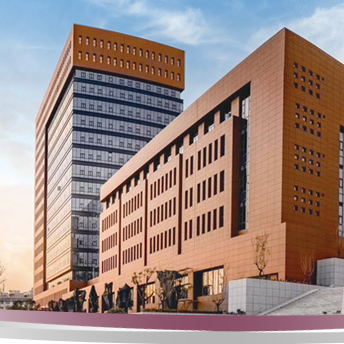
\includegraphics[width=1\linewidth]{hutb_building.png}
        \caption{bbb}
        \end{minipage}
    \end{subfigure}
    \caption{图片竖排多图横排布局}
    \label{f.csu_col_row}
\end{figure}

竖排多图横排布局如图\ref{f.csu_col_row}所示。注意看(a)、(b)编号与图关系


\section{横排多图竖排布局}

潮涌湘江阔,鹏翔天地宽。湖南工商大学正以习近平新时代中国特色社会主义思想为指引,秉持“新工科+新商科+新文科”与理科融合发展的思路,努力形成一流的理念、一流的目标、一流的标准、一流的质量、一流的机制,打造创新工商、人文工商、艺术工商、体育工商、数智工商、绿色工商、幸福工商,建设读书求知的好园地,乘高等教育改革奋进的东风,朝着创新型一流工商大学的愿景扬帆远航。

\begin{figure}[!htb]
    \centering
    \begin{subfigure}[t]{0.3\linewidth}
        \captionsetup{justification=centering} 
        \begin{minipage}[b]{1\linewidth}
        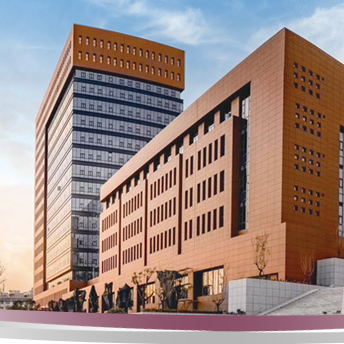
\includegraphics[width=0.45\linewidth]{hutb_building.png}
        \includegraphics[width=0.45\linewidth]{hutb_eim.png}
        \caption{}
        \end{minipage}
    \end{subfigure}\\
    \begin{subfigure}[t]{0.3\linewidth}
        \captionsetup{justification=centering} 
        \begin{minipage}[b]{1\linewidth}
        \includegraphics[width=0.45\linewidth]{hutb_eim.png}
        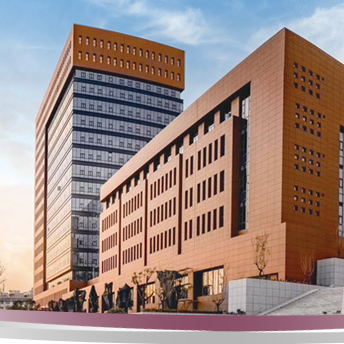
\includegraphics[width=0.45\linewidth]{hutb_building.png}
        \caption{}
        \end{minipage}
    \end{subfigure}
    \caption{图片横排多图竖排布局}
    \label{f.csu_row_col}
\end{figure}

横排多图竖排布局如图\ref{f.csu_row_col}所示。注意看(a)、(b)编号与图关系。

\newpage
%%%%%%%%%%%%%%%%%%%%%%%%%%%%%%%%图像插入示例%%%%%%%%%%%%%%%%


%%%%%%%%%%%%%%%%%%%%%%%%%%%%%%%%表格插入示例%%%%%%%%%%%%%%%%
%!TEX root = ../../csuthesis_main.tex
\chapter{表格插入示例}

\begin{table}[htb]
  \centering
  \caption{学校文件里对表格的要求不是很高,不过按照学术论文的一般规范,表格为三线表。}
  \label{T.example}
  \begin{tabular}{llllll}
  \hline
   & A  & B  & C  & D  & E \\
  \hline
1 	& 212 & 414 & 4 		& 23 & fgw	\\
2 	& 212 & 414 & v 		& 23 & fgw	\\
3 	& 212 & 414 & vfwe		& 23 & 嗯	\\
4 	& 212 & 414 & 4fwe		& 23 & 嗯	\\
5 	& af2 & 4vx & 4 		& 23 & fgw	\\
6 	& af2 & 4vx & 4 		& 23 & fgw	\\
7 	& 212 & 414 & 4 		& 23 & fgw	\\

\hline{}
\end{tabular}
\end{table}

\textbf{表格如表\ref{T.example}所示,latex表格技巧很多,这里不再详细介绍。}

潮涌湘江阔,鹏翔天地宽。湖南工商大学正以习近平新时代中国特色社会主义思想为指引,秉持“新工科+新商科+新文科”与理科融合发展的思路,努力形成一流的理念、一流的目标、一流的标准、一流的质量、一流的机制,打造创新工商、人文工商、艺术工商、体育工商、数智工商、绿色工商、幸福工商,建设读书求知的好园地,乘高等教育改革奋进的东风,朝着创新型一流工商大学的愿景扬帆远航。


\newpage

\chapter{公式插入示例}

潮涌湘江阔,鹏翔天地宽。湖南工商大学正以习近平新时代中国特色社会主义思想为指引,秉持“新工科+新商科+新文科”与理科融合发展的思路,努力形成一流的理念、一流的目标、一流的标准、一流的质量、一流的机制,打造创新工商、人文工商、艺术工商、体育工商、数智工商、绿色工商、幸福工商,建设读书求知的好园地,乘高等教育改革奋进的东风,朝着创新型一流工商大学的愿景扬帆远航。


\textbf{公式插入示例如公式(\ref{E.example})所示。}

\begin{equation}
\gamma_{x}=
\left\{
  \begin{array}{lr}
  0, & {\rm if}~~\;|x| \leq \delta \\
  x, & {\rm otherwise}
  \end{array}
\right.
\label{E.example}
\end{equation}


\newpage
%%%%%%%%%%%%%%%%%%%%%%%%%%%%%%%%表格插入示例%%%%%%%%%%%%%%%%


%%%%%%%%%%%%%%%%%%%%%%%%%%%%%%%%参考文献插入示例%%%%%%%%%%%%%%%%
%!TEX root = ../../csuthesis_main.tex
\chapter{引用文献标注}

文献标注和索引的处理一直是学术写作的一个麻烦事,特别是在word环境下。latex中我们只需要
编辑(或直接获取) BibTeX 格式索引文件然后在正文中使用\cs{cite} \cs{citet}等指令
进行引用标注就可以。下面介绍在文章中引用指令的具体使用方法。

\section{顺序编码}

根据学校要求,参考文献标注用中括号上标形式进行标注。使用方式与效果如下表所展示

\begin{tabular}{l@{\quad$\Rightarrow$\quad}l}
    \verb|\cite{knuth1984texbook}|               & \cite{knuth1984texbook}               \\
    \verb|\citet{knuth1984texbook}|              & \citet{knuth1984texbook}              \\
    \verb|\citep{knuth1984texbook}|              & \citep{knuth1984texbook}              \\
    % 暂不支持
    % \verb|\cite[42]{knuth1984texbook}|           & \cite[42]{knuth1984texbook}           \\
    \verb|\cite{knuth1984texbook,lamport1994latex}| & \cite{knuth1984texbook,lamport1994latex} \\
\end{tabular}

\section{获取BibTeX格式索引}

获取参考文献的 BibTeX 格式索引有两种方式

\begin{itemize}
    \item 通过Google Scholare或者百度学术等学术文献搜索引擎获取,自行编辑 .bib 文件
    \item 通过Zotero等学术文献整理软件,添加所有的引用文献至库中,导出对应的 .bib 文件
\end{itemize}

编译带参考文献的文章时,我们需要两次编译过程。我们提供了对应的自动化脚本,以及配合vscode latex插件的任务流程,
帮助模板使用者进行编译。

\section{参考文献插入示例}

LaTeX\cite{lamport1994latex}插入参考文献最方便的方式是使用bibliography\cite{pritchard1969statistical},大多数出版商的论文页面\cite{lamport1994latex,pritchard1969statistical}都会有导出bib格式参考文献的链接,把每个文献的bib放入``hutbthesis\_main.bib'',然后用bibkey即可插入参考文献。

潮涌湘江阔,鹏翔天地宽。湖南工商大学正以习近平新时代中国特色社会主义思想为指引,秉持“新工科+新商科+新文科”与理科融合发展的思路,努力形成一流的理念、一流的目标、一流的标准、一流的质量、一流的机制,打造创新工商、人文工商、艺术工商、体育工商、数智工商、绿色工商、幸福工商,建设读书求知的好园地,乘高等教育改革奋进的东风,朝着创新型一流工商大学的愿景扬帆远航。

\newpage




%%%%%%%%%%%%%%%%%%%%%%%%%%%%%%%%参考文献插入示例%%%%%%%%%%%%%%%%

%%%%%%%%%%%%%%%%%%%%%%%%%%%%%%%%总结插入示例%%%%%%%%%%%%%%%%
%!TEX root = ../../csuthesis_main.tex

%%%%%%%%%%%%%%%%%%%%%%%%%%%%%%%%总结插入示例%%%%%%%%%%%%%%%%



%!TEX root = ../../csuthesis_main.tex
\chapter{一级标题}

这是湖南工商大学学位论文\LaTeX{}模板,下面的文字主要作用为对重构后的模板样式设置进行测试。
测试样例基本覆盖模板设定,包括多级标题的基本样式,段落与缩进距离。

\section{二级标题}

\subsection{三级标题}

\subsubsection{四级标题}

一级标题根据学校提供的Word模板要求,三号黑体居中,上下各空一行,章节号空一个汉字,
并且每一章节单独起一页,章节号格式应使用阿拉伯数字而非中文汉字。

二级标题为小四号黑体,缩进两个汉字。章节号后空一个汉字。

三级标题小四号楷体GB2312,字体包含在项目中,同样缩进两个汉字,章节号后空一个汉字。

四级标题参照本科学术论文设计样式,分项采取(1)、(2)、(3)的序号。

所有标题样式由\cls{undergraduate.cls}模板文件 \cs{ctexset} 进行设置。

\section{字体}

正文字体默认使用小四号宋体,英文为小四号 Times New Romen,各段行首缩进两个汉字

承千年文脉,扬湖湘精神。湖南工商大学坐落在历史文化名城长沙,创建于1949年,享有“经济湘军基地,企业名家摇篮”的盛誉。她是一所院士领衔的涵盖管理学、经济学、工学、理学、法学、文学、艺术学、交叉学科等多学科相互支撑、协调发展、特色鲜明的财经类大学,是湖南省本科一批招生高校、教育部本科教学工作水平评估优秀高校、博士学位授予立项建设单位、“十三五”国家产教融合发展工程应用型本科高校、全国首批百强“深化创新创业教育改革示范高校”、全国高校实践育人创新创业基地、教育部人文社会科学优秀成果奖大满贯高校。

学校拥有一批以中国工程院院士陈晓红为代表,包括国务院学位委员会管理科学与工程学科评议组召集人、国家自然科学基金委员会委员、教育部管理科学与工程类专业教学指导委员会副主任委员、教育部科技委管理学部副主任、国家基础科学中心主任、国家一级重点学科“管理科学与工程”和国家自然科学基金委创新研究群体负责人、教育部“长江学者创新团队”首席教授、国家“万人计划”领军人才、全国文化名家暨“四个一批”人才、国家首批“百千万人才工程”第一层次人选等在内的国家级高层次人才;拥有高级职称教师近500人,具有博士学位教师近800人;引智院士9名、“杰青”“长江”等专家学者和优秀企业家70人;院士团队入选“全国高校黄大年式教师团队”。

英文字体展示如下:

TeX (/tɛx, tɛk/, see below), stylized within the system as TEX, is a typesetting system (or a "formatting system") which was designed and mostly written by Donald Knuth\cite{knuth1984texbook} and released in 1978. TeX is a popular means of typesetting complex mathematical formulae; it has been noted as one of the most sophisticated digital typographical systems.


\subsection{调节字号}

可以使用 \cs{zihao}命令来调节字号。

\begin{tabular}{ll}
  \verb|\zihao{3} | & \zihao{3}  三号字 English \\
  \verb|\zihao{-3}| & \zihao{-3} 小三号 English \\
  \verb|\zihao{4} | & \zihao{4}  四号字 English \\
  \verb|\zihao{-4}| & \zihao{-4} 小四号 English \\
  \verb|\zihao{5} | & \zihao{5}  五号字 English \\
  \verb|\zihao{-5}| & \zihao{-5} 小五号 English \\
\end{tabular}

\subsection{调节字体}

需要说明的是由于学校写作指导要求的字体部分不可在Linux上使用,即便你的写作过程是在Linux或者macOS上完成的,
我们仍\textbf{强烈建议}您在Windows操作系统上编译最终版论文。

中文字体可以使用如下命令来调节。

\begin{tabular}{l l}
  \verb|\songti| & {\songti 宋体} \\
  \verb|\heiti| & {\heiti 黑体} \\
%   \verb|\kaiti| & {\kaiti 楷体}
\end{tabular}


\section{模板主要结构}

本项目模板的主要结构, 如下表所示:
% TODO 进一步完善

\begin{table}[ht]
  \centering
  \begin{tabular}{r|l|l}
    \hline\hline
    \multicolumn{2}{l|}{csuthesis\_main.tex } & 主文档,可以理解为文章入口。                                      \\ \hline
                                                & info.tex   & 作者、文章基本信息 \\ \cline{2-3}
                                                & abstactzh/en.tex    & 中/英文摘要内容 \\ \cline{2-3}
    \raisebox{1em}{content 目录 }          &  subchapters 目录   & 章节内容           \\ \hline
    \multicolumn{2}{l|}{images 目录}         & 用于存放图片文件                                                \\ \hline
    \multicolumn{2}{l|}{hutbthesis.cls }       & 模板入口                         \\ \hline\hline
  \end{tabular}
\end{table}

我们不建议模板使用者更改原有模板的结构,
但如果您确实需要,请务必先充分阅读本模板的使用说明并了解相应的\LaTeX{}模板设计知识。

%!TEX root = ../../csuthesis_main.tex
\chapter{图表示例}

\section{图片与布局}

\subsection{插图}

图片可以通过\cs{includegraphics}指令插入,我们建议模板使用者将文章所需插入的图片源问卷放置在 images 目录中,
另外,矢量图片应使用PDF格式,位图照片则应使用JPG格式(LaTeX不支持TIFF格式)。具有透明背景的栅格图可以使用PNG格式。

下面是一个简单的插图示例。

\begin{figure}[hbt]
    \centering
    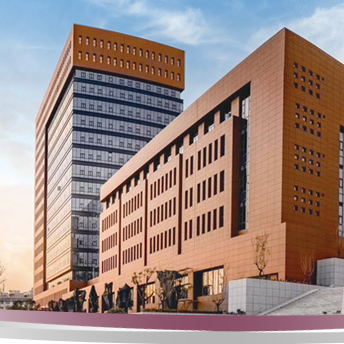
\includegraphics[width=0.3\linewidth]{hutb_building.png}
    \caption{插图示例}
    \label{f.example}
\end{figure}


如果一个图由多个分图(子图)组成,应通过(a),(b),(c)进行标识并附注在分图(子图下方)。
目前子图标识不居中问题没有解决,预计下个版本修复。

\subsection{横向布局}

模板提供常见的图片布局,比如单图布局\ref{f.example},另外还有横排布局如下:

\begin{figure}[!htb]
    \centering
    \begin{subfigure}[t]{0.24\linewidth}
        \begin{minipage}[b]{1\linewidth}
        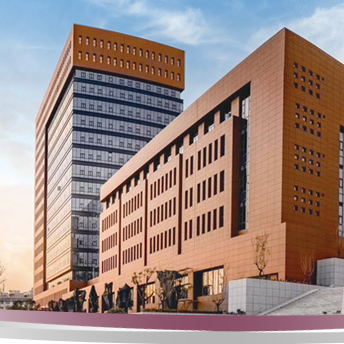
\includegraphics[width=1\linewidth]{hutb_building.png}
        \caption{test}
        \end{minipage}
    \end{subfigure}
    \begin{subfigure}[t]{0.24\linewidth}
        \begin{minipage}[b]{1\linewidth}
        \includegraphics[width=1\linewidth]{hutb_eim.png}
        \caption{test}
        \end{minipage}
    \end{subfigure}
    \begin{subfigure}[t]{0.24\linewidth}
        \begin{minipage}[b]{1\linewidth}
        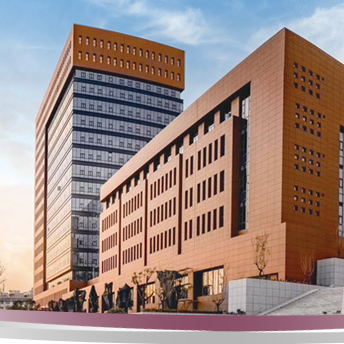
\includegraphics[width=1\linewidth]{hutb_building.png}
        \caption{test}
        \end{minipage}
    \end{subfigure}
    \begin{subfigure}[t]{0.24\linewidth}
        \begin{minipage}[b]{1\linewidth}
        \includegraphics[width=1\linewidth]{hutb_eim.png}
        \caption{test}
        \end{minipage}
    \end{subfigure}
    \caption{图片横排布局示例}
    \label{f.row}
\end{figure}

\section{纵向布局}

纵向布局如图\ref{f.col}

\begin{figure}[!htb]
    \centering
    \begin{subfigure}[t]{0.15\linewidth}
        \captionsetup{justification=centering} %ugly hacks
        \begin{minipage}[b]{1\linewidth}
        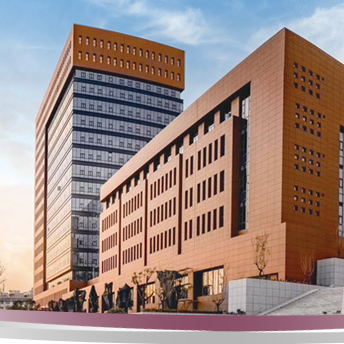
\includegraphics[width=1\linewidth]{hutb_building.png}
        \caption{test}
        \end{minipage}
    \end{subfigure}\\
    \begin{subfigure}[t]{0.15\linewidth}
        \captionsetup{justification=centering} %ugly hacks
        \begin{minipage}[b]{1\linewidth}
        \includegraphics[width=1\linewidth]{hutb_eim.png}
        \caption{test}
        \end{minipage}
    \end{subfigure}
    \caption{图片纵向布局示例}
    \label{f.col}
\end{figure}

\section{竖排多图横排布局}

\begin{figure}[!htb]
    \centering
    \begin{subfigure}[t]{0.13\linewidth}
        \captionsetup{justification=centering} 
        \begin{minipage}[b]{1\linewidth}
        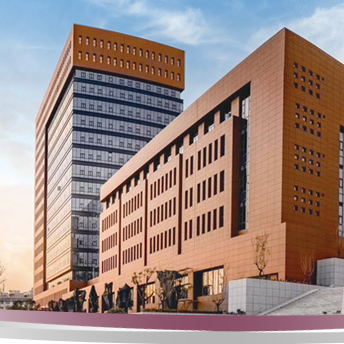
\includegraphics[width=1\linewidth]{hutb_building.png} 
        \vspace{-1ex} \vfill
        \includegraphics[width=1\linewidth]{hutb_eim.png}
        \caption{aaa}
        \end{minipage}
    \end{subfigure}
    \begin{subfigure}[t]{0.13\linewidth}
        \captionsetup{justification=centering} 
        \begin{minipage}[b]{1\linewidth}
        \includegraphics[width=1\linewidth]{hutb_eim.png} 
        \vspace{-1ex} \vfill
        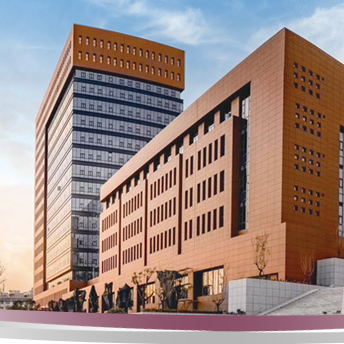
\includegraphics[width=1\linewidth]{hutb_building.png}
        \caption{bbb}
        \end{minipage}
    \end{subfigure}
    \caption{图片竖排多图横排布局}
    \label{f.csu_col_row}
\end{figure}

竖排多图横排布局如图\ref{f.csu_col_row}所示。注意看(a)、(b)编号与图关系


\section{横排多图竖排布局}

潮涌湘江阔,鹏翔天地宽。湖南工商大学正以习近平新时代中国特色社会主义思想为指引,秉持“新工科+新商科+新文科”与理科融合发展的思路,努力形成一流的理念、一流的目标、一流的标准、一流的质量、一流的机制,打造创新工商、人文工商、艺术工商、体育工商、数智工商、绿色工商、幸福工商,建设读书求知的好园地,乘高等教育改革奋进的东风,朝着创新型一流工商大学的愿景扬帆远航。

\begin{figure}[!htb]
    \centering
    \begin{subfigure}[t]{0.3\linewidth}
        \captionsetup{justification=centering} 
        \begin{minipage}[b]{1\linewidth}
        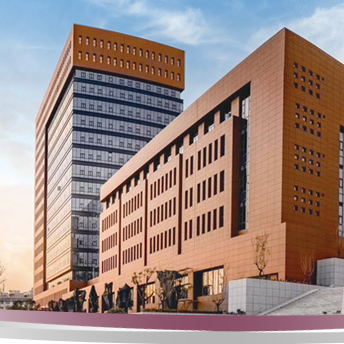
\includegraphics[width=0.45\linewidth]{hutb_building.png}
        \includegraphics[width=0.45\linewidth]{hutb_eim.png}
        \caption{}
        \end{minipage}
    \end{subfigure}\\
    \begin{subfigure}[t]{0.3\linewidth}
        \captionsetup{justification=centering} 
        \begin{minipage}[b]{1\linewidth}
        \includegraphics[width=0.45\linewidth]{hutb_eim.png}
        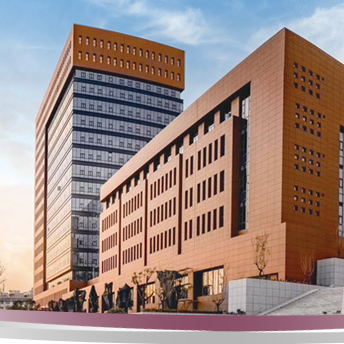
\includegraphics[width=0.45\linewidth]{hutb_building.png}
        \caption{}
        \end{minipage}
    \end{subfigure}
    \caption{图片横排多图竖排布局}
    \label{f.csu_row_col}
\end{figure}

横排多图竖排布局如图\ref{f.csu_row_col}所示。注意看(a)、(b)编号与图关系。

\newpage
%!TEX root = ../../csuthesis_main.tex
\chapter{表格插入示例}

\begin{table}[htb]
  \centering
  \caption{学校文件里对表格的要求不是很高,不过按照学术论文的一般规范,表格为三线表。}
  \label{T.example}
  \begin{tabular}{llllll}
  \hline
   & A  & B  & C  & D  & E \\
  \hline
1 	& 212 & 414 & 4 		& 23 & fgw	\\
2 	& 212 & 414 & v 		& 23 & fgw	\\
3 	& 212 & 414 & vfwe		& 23 & 嗯	\\
4 	& 212 & 414 & 4fwe		& 23 & 嗯	\\
5 	& af2 & 4vx & 4 		& 23 & fgw	\\
6 	& af2 & 4vx & 4 		& 23 & fgw	\\
7 	& 212 & 414 & 4 		& 23 & fgw	\\

\hline{}
\end{tabular}
\end{table}

\textbf{表格如表\ref{T.example}所示,latex表格技巧很多,这里不再详细介绍。}

潮涌湘江阔,鹏翔天地宽。湖南工商大学正以习近平新时代中国特色社会主义思想为指引,秉持“新工科+新商科+新文科”与理科融合发展的思路,努力形成一流的理念、一流的目标、一流的标准、一流的质量、一流的机制,打造创新工商、人文工商、艺术工商、体育工商、数智工商、绿色工商、幸福工商,建设读书求知的好园地,乘高等教育改革奋进的东风,朝着创新型一流工商大学的愿景扬帆远航。


\newpage

\chapter{公式插入示例}

潮涌湘江阔,鹏翔天地宽。湖南工商大学正以习近平新时代中国特色社会主义思想为指引,秉持“新工科+新商科+新文科”与理科融合发展的思路,努力形成一流的理念、一流的目标、一流的标准、一流的质量、一流的机制,打造创新工商、人文工商、艺术工商、体育工商、数智工商、绿色工商、幸福工商,建设读书求知的好园地,乘高等教育改革奋进的东风,朝着创新型一流工商大学的愿景扬帆远航。


\textbf{公式插入示例如公式(\ref{E.example})所示。}

\begin{equation}
\gamma_{x}=
\left\{
  \begin{array}{lr}
  0, & {\rm if}~~\;|x| \leq \delta \\
  x, & {\rm otherwise}
  \end{array}
\right.
\label{E.example}
\end{equation}


\newpage
%!TEX root = ../../csuthesis_main.tex
\chapter{引用文献标注}

文献标注和索引的处理一直是学术写作的一个麻烦事,特别是在word环境下。latex中我们只需要
编辑(或直接获取) BibTeX 格式索引文件然后在正文中使用\cs{cite} \cs{citet}等指令
进行引用标注就可以。下面介绍在文章中引用指令的具体使用方法。

\section{顺序编码}

根据学校要求,参考文献标注用中括号上标形式进行标注。使用方式与效果如下表所展示

\begin{tabular}{l@{\quad$\Rightarrow$\quad}l}
    \verb|\cite{knuth1984texbook}|               & \cite{knuth1984texbook}               \\
    \verb|\citet{knuth1984texbook}|              & \citet{knuth1984texbook}              \\
    \verb|\citep{knuth1984texbook}|              & \citep{knuth1984texbook}              \\
    % 暂不支持
    % \verb|\cite[42]{knuth1984texbook}|           & \cite[42]{knuth1984texbook}           \\
    \verb|\cite{knuth1984texbook,lamport1994latex}| & \cite{knuth1984texbook,lamport1994latex} \\
\end{tabular}

\section{获取BibTeX格式索引}

获取参考文献的 BibTeX 格式索引有两种方式

\begin{itemize}
    \item 通过Google Scholare或者百度学术等学术文献搜索引擎获取,自行编辑 .bib 文件
    \item 通过Zotero等学术文献整理软件,添加所有的引用文献至库中,导出对应的 .bib 文件
\end{itemize}

编译带参考文献的文章时,我们需要两次编译过程。我们提供了对应的自动化脚本,以及配合vscode latex插件的任务流程,
帮助模板使用者进行编译。

\section{参考文献插入示例}

LaTeX\cite{lamport1994latex}插入参考文献最方便的方式是使用bibliography\cite{pritchard1969statistical},大多数出版商的论文页面\cite{lamport1994latex,pritchard1969statistical}都会有导出bib格式参考文献的链接,把每个文献的bib放入``hutbthesis\_main.bib'',然后用bibkey即可插入参考文献。

潮涌湘江阔,鹏翔天地宽。湖南工商大学正以习近平新时代中国特色社会主义思想为指引,秉持“新工科+新商科+新文科”与理科融合发展的思路,努力形成一流的理念、一流的目标、一流的标准、一流的质量、一流的机制,打造创新工商、人文工商、艺术工商、体育工商、数智工商、绿色工商、幸福工商,建设读书求知的好园地,乘高等教育改革奋进的东风,朝着创新型一流工商大学的愿景扬帆远航。

\newpage




%!TEX root = ../../csuthesis_main.tex


% % 主文件有代码去掉页眉章节编号的“.”,但这会因为bug导致无编号章节显示一个错误编号,所以这里在无编号章节之前再次重定义sectionmark。
% \renewcommand{\sectionmark}[1]{\markright{#1}}


%%%%%%%%%%%%%%%%%%%%%%%%%%%%%%%%%%%%%%%%%%%%%%%%%%
% 致谢
%
% 存储在\content\acknowledgements.tex文件中
% 根据本科生院的要求,致谢应该在参考文献的前面,不编章号,而附录应该位于参考文献后。
%%%%%%%%%%%%%%%%%%%%%%%%%%%%%%%%%%%%%%%%%%%%%%%%%%
%!TEX root = ../csuthesis_main.tex
\begin{acknowledgements} 

感谢制作出中南大学本科学位论文 LaTeX 模板的edwardzcn。

感谢制作出中南大学博士学位论文 LaTeX 模板的郭大侠@CSGrandeur。

感谢添加本科学位论文样式支持的@BlurryLight。

感谢帮助重构项目并进行测试的@burst-bao以及为独立使用LaTeX进行毕业论文写作提供宝贵经验的16级的姜析阅学长。

感谢 CTeX-kit 提供了 LaTeX 的中文支持。

感谢上海交通大学学位论文 LaTeX 模板的维护者们 @sjtug 和清华大学学位论文 LaTeX 模板的维护者们 @tuna 给予的宝贵设计经验。

感谢所有为模板贡献过代码的同学们!

\end{acknowledgements}


%%%%%%%%%%%%%%%%%%%%%%%%%%%%%%%%%%%%%%%%%%%%%%%%%%
% 参考文献
%
% 存储在\content\acknowledgements.tex文件中
% 根据本科生院的要求,致谢应该在参考文献的前面,不编章号,而附录应该位于参考文献后。
% 有待修复
%%%%%%%%%%%%%%%%%%%%%%%%%%%%%%%%%%%%%%%%%%%%%%%%%%
% \section{参考文献} % bibliography会自动显示参考文献四个字
\addcontentsline{toc}{chapter}{参考文献} % 由于参考文献不是chapter,这句把参考文献加入目录
% \nocite{*} % 该命令用于显示全部参考文献,即使文中没引用
% cls文件中已经引入package,这里不需要调用 \bibliographystyle 了。
%\bibliographystyle{gbt7714-2005}
%\bibliography{reference}

\printbibliography

%\bibliography{hutbtheisi_main}
\newpage


%%%%%%%%%%%%%%%%%%%%%%%%%%%%%%%%%%%%%%%%%%%%%%%%%%
% 附录部分
%
% 根据学校要求,正文中不应出现长篇幅的代码段或公式推证
% 应单独放置在正文后的附录部分
%%%%%%%%%%%%%%%%%%%%%%%%%%%%%%%%%%%%%%%%%%%%%%%%%%

% https://www.zhihu.com/question/29413517/answer/44358389 %
% 说明如下:
% secnumdepth 这个计数器是 LaTeX 标准文档类用来控制章节编号深度的。
% 在 article 中,这个计数器的值默认是 3,对应的章节命令是 \subsubsection。
% 也就是说,默认情况下,article 将会对 \subsubsection 及其之上的所有章节标题进行编号,也就是 \part, \section, \subsection, \subsubsection。LaTeX 标准文档类中,最大的标题是 \part。它在 book 和 report 类中的层级是「-1」,在 article 类中的层级是「0」。这里,我们在调用 \appendix 的时候将计数器设置为 -2,因此所有的章节命令都不会编号了。不过,一般还是会保留 \part 的编号的。所以在实际使用中,将它设置为 0 就可以了。

% 在修改过程中请注意不要破环命令的完整性

% \renewcommand\appendix{\setcounter{secnumdepth}{-2}}
\appendix
%!TEX root = ../csuthesis_main.tex
% \begin{appendixs} % 无章节编号
\chapter{附录代码}

附录部分用于存放这里用来存放不适合放置在正文的大篇幅内容、典型如代码、图纸、完整数学证明过程等内容。

\section{堆溢出检测算法}

\begin{algorithm}[h]
    \caption{堆溢出检测算法}\label{alg:ovf}
    \begin{algorithmic}[1]
        \IF {$\beta \in \mathbb{N^{*}} \land \Delta_\beta = \Delta_{\beta - 1} \land \beta < S$}
            \STATE 正常写入
        \ELSIF {$\beta \in \mathbb{N^{*}} \land \Delta_\beta \neq \Delta_{\beta - 1} \land \beta \geq S$}
            \STATE 发生堆溢出
        \ENDIF
    \end{algorithmic}
\end{algorithm}

\section{KMP算法C++描述}

% \begin{minted}[linenos]{c}
\begin{lstlisting}
    const int maxn=2e5+5; 
    int nt[maxn];
    int aa[maxn],bb[maxn];
    int a[maxn],b[maxn];
    int n;
    //参数为模板串和next数组
    //字符串均从下标0开始
    void kmpGetNext(int *s,int *Next)
    {
        Next[0]=0;
    //    int len=strlen(s);
        for(int i=1,j=0;i<n;i++)
        {
            while(j&&s[i]!=s[j]) j=Next[j];
            if(s[i]==s[j]) j++;
            Next[i+1]=j;
        }
    //    Next[len]=0;
    }
    int kmp(int *ss,int *s,int *Next)
    {
        kmpGetNext(s,Next);
    //  调试输出Next数组
    //	int len=strlen(s);
    //	for(int i=0;i<=n;i++)
    //		cout<<Next[i]<<" ";
    //	cout<<endl; 
    
    //    int ans=0;
    //    int len1=strlen(ss);
    //    int len2=strlen(s);
        for(int i=0,j=0;i<2*n;i++)  //倍长 
        {
            while(j&&ss[i%n]!=s[j])j=Next[j];
            if(ss[i%n]==s[j]) j++;
            if(j==n){
                return 1;
            }
               
        }
        return 0;
    }
    int main(void)
    {
        while(cin>>n)
        {
            memset(a,0,sizeof(a));
            memset(b,0,sizeof(b));
            rep(i,0,n) cin>>aa[i];
            rep(i,0,n) cin>>bb[i];
            sort(aa,aa+n);
            sort(bb,bb+n);
            rep(i,0,n-1){
                a[i]=aa[i+1]-aa[i];
                b[i]=bb[i+1]-bb[i];
            }
            a[n-1]=360000+aa[0]-aa[n-1];
    //		rep(i,0,n) cout<<a[i]<<" ";
    //		cout<<endl;
            b[n-1]=360000+bb[0]-bb[n-1];
    //		rep(i,0,n) cout<<b[i]<<" ";
    //		cout<<endl;
            if(kmp(a,b,nt))
                cout<<"possible"<<endl;
            else cout<<"impossible"<<endl;
        }
        return 0;
    }
\end{lstlisting}
% \end{minted}

\chapter{康托尔辩辞录:数学的自由与制约}

(录自康托尔:《一般集合论基础》,1883)

数学在其发展中是完全自由的,它只受下述自明的关注所制约,即它的概念既要内在地不存在矛盾,还要参与确定与此前形成的,已经存在着地和已被证明地概念之关系(借助定义贯串起来)。特别地,在引入新数时,数学只遵循:在给出它们地定义时使之具有某种确定性,并且在某些情况下,使之与老数有某种关系,在特定地场合中这种关系一定会使它们(新数和老数)互相区别开来,只要一个数满足这些条件,数学只能而且必须把它看作是存在的和实在的东西,这正是我……关于为什么必须把有理数、无理数和复数看作与有限正整数一样是实在的所建议的理由。

我相信,没有必要害怕,许多人是害怕,这些原则含有对于科学的危险,一方面,实行造出新数的自由必须服从所设计的条件,但这些条件给任意性留下的活动空间是非常小的。而且,每一数学概念在其自身之中也带有必要的矫正物;如果它没有收获也不合适(它的无用很快就会表明这一点),那么它将由于没有成功而被丢弃。另一方面,在我看来,对于数学研究工作的任何多余的限制只会随之而带来更大的危险,由于实际上并没有任何理由可说明它是由科学的本质推断出来的,它的危险就更大了,而数学的本质恰恰在于它的自由。

如果高斯、柯西、阿贝尔、雅可比、狄利克雷、魏尔斯特拉斯、埃尔米特和黎曼总是被束缚而拿他们的新想法去臣服于形而上学的控制,那么,我们今日就不可能为现代函数论的雄伟建筑而高兴,现代函数论的设计和矗立是完全自由的,毫无短视的瞬间目的……。如果福克斯、庞加莱和其他许多杰出的智者受外来影响所包围和限制,我们就会见不到他们带给微分方程论的巨大的推动,还有,如果枯莫尔不是斗胆地(大有仿效者)把所谓的“理想”数引入数论,我们今天也无从去羡慕钦佩克罗内克和戴德金在代数和算术上十分重要和杰出的工作。

因此,如已说明的,数学是要脱离形而上学的桎梏而完全自由地发展 \dots



% \end{appendixs}



\end{document}
